%\documentclass[11pt,a4paper]{scrartcl}
\documentclass[12pt]{article}

\usepackage[top=2.0cm, right=2.0cm, left=2.0cm, bottom=2.0cm]{geometry}
\usepackage[utf8]{inputenc}
\usepackage[french]{babel}
%tableau
\usepackage{array, multirow}
%graphs
\usepackage{graphicx}
\usepackage{float, caption}
\usepackage{amsmath,amssymb,mathrsfs}
\usepackage{pgf}
\usepackage{tikz}
\usetikzlibrary{arrows,shapes}
                                                                                                               
\usepackage [tikz]{bclogo}                                                                                          
      

\usepackage{natbib}
%pour avoir la biblio avec nom d'auteur et année dans le texte
\bibpunct{(}{)}{;}{a}{,}{,}
%pour avoir les reference entre parenthese et en cas de ref multiple séparé par des ;
\sloppy 
%utiliser ca si latex trop exigeant en largeur ligne

\title{Comprendre les épidémies et l'évolution de la virulence avec \textit{Evolvir}}
\author{Sébastien Ballesteros$^{1}$}

\date{}

\begin{document}

\maketitle

~ \\
$^1$UMR 7625 (UPMC, ENS, AgroParisTech, CNRS), Ecole Normale
Supérieure, Équipe Eco-Evolution Mathématiques, 46 rue d'Ulm,
F-75230 Paris Cedex 05, France. \
~ \\


\begin{center}
  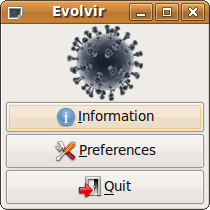
\includegraphics[]{graph/welcome.png}
\end{center}

\tableofcontents


\clearpage

\section{Préambule}

\textit{Evolvir} est un logiciel libre sous les termes de la Licence
Publique Générale GNU tel que publiée par la Free Software Foundation.

Il est dévelopé en language C et fait appel à la librairie GTK.

\textit{Evolvir} est distribué dans l'espoir qu'il puisse être utile
mais sans aucune garantie ; sans même une garantie implicite de valeur
marchande ou d'adéquation à un besoin particulier.  Voir la Licence
Publique Générale GNU pour plus d'informations.


\section{Dynamique épidémiologique}


La dynamique épidémiologique caractérise la démographie d'une maladie
infectieuse (le nombre de cas, la durée, etc.)

\subsection{Modéliser une épidémie avec \textit{Evolvir}: cas des contacts locaux}

Considérons un cas simple (figure \ref{fig:selecao}): un individu
infecté par une maladie infectieuse est entouré de voisins non
malades. Notre individu infecté va pouvoir transmettre la maladie à
ses voisins. Le hasard fait partie de ce processus et, il se peut que
par chance, les voisins échappent à la contamination. Les voisins
ayant été infecté vont ensuite à leur tour être malade et continuer à
transmettre la maladie. Il se peut encore que par chance, la chaîne de
transmission s'interrompt et que la maladie disparaisse.

\textit{Evolvir} permet de simuler ce processus d'infection, tenant
compte du jeu du hasard ainsi que de deux autres processus :
\begin{itemize}
\item la mort de l'individu suite à la maladie (pour simplifier on
  considérera que tous les individus malades succomberont à leur
  maladie mais au bout d'un temps variable) ;
\item le remplacement des morts par de nouveaux individus sains que
  cela soit due à des naissances ou à de l'immigration.
\end{itemize}

\begin{figure}[h!]
  \center
	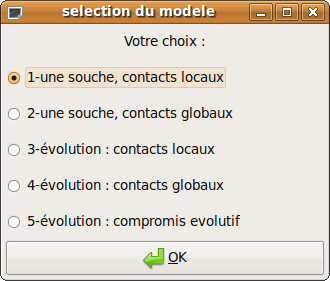
\includegraphics[width=0.4\linewidth]{graph/selecao.png}
        \caption{Choix du modèle: sélectionner le premier choix
          conduit à simuler une épidémie dont les contacts ont lieux
          de proche en proche.}
\label{fig:selecao}
\end{figure}

La prise en compte de ces trois processus (infections, morts et
renouvellement des individus susceptibles à la maladie) avec
\textit{Evolvir} nous permet d'observer l'éventuel développement d'une
épidémie pour différentes maladies. Nous caractériserons les maladies
par deux paramètres : la transmission et la virulence (figure
\ref{fig:parametres}).

\begin{figure}[h!]
  \center
	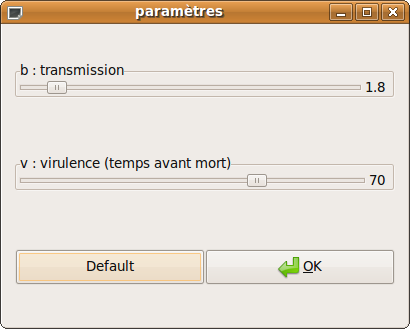
\includegraphics[width=0.4\linewidth]{graph/parametres.png}
        \caption{Sélection des paramètres, notez que la virulence est
          exprimée ici comme le temps pendant lequel un hôte infecté
          reste en vie. Une forte valeur de ce paramètre correspond
          donc à un agent infectieux peu virulent, tandis qu'une
          faible valeur représente un agent infectieux tuant très
          rapidement les individus malades et donc très virulent.}
\label{fig:parametres}
\end{figure}

Après avoir sélectionné des paramètres (ou choisi ceux proposés par
défaut), il reste à valider et à se laisser guider par les boites de
dialogues d'\textit{Evolvir} jusqu'à la fenêtre de visualisation de
l'épidémie (figure \ref{fig:evolvir}).

\begin{figure}[h!]
  \center
	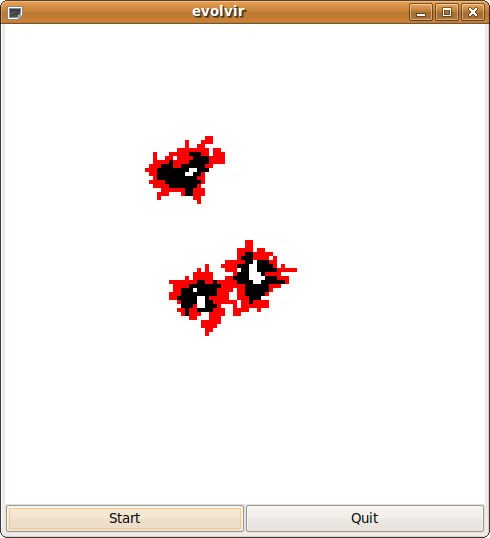
\includegraphics[width=0.4\linewidth]{graph/evolvir.png}
        \caption{Dynamique épidémiologique: les couleurs représentent
          différentes catégories d'individus. Blanc : individus
          susceptibles ; rouge : individus malades ; noir : individus
          morts.}
\label{fig:evolvir}
\end{figure}

                                                                                                                
\begin{bclogo}[couleur = gray!30, logo = \bclampe , barre =                                                      
none, noborder=true ]{Simulation}                                                                                  

En choisissant différentes valeurs de paramètres, déterminez les
valeurs de transmission et de virulence pour qu'une épidémie puisse
débuter, persister dans une population ou bien se développer puis
s'éteindre (figure \ref{fig:evolvir}).

\end{bclogo}                                                                                                        


\subsection{Une grande ville : contacts globaux}

L'hypothèse des contacts locaux n'est pas toujours réaliste. Dans une
grande ville par exemple, il peut être plus pertinent de supposer que
les habitants peuvent potentiellement tous se rencontrer et pas
seulement leurs voisin (pensez par exemple aux transports en commun).

                                                                                                                
\begin{bclogo}[couleur = gray!30, logo = \bclampe , barre =                                                      
none, noborder=true ]{Simulation}                                                                                  

\textit{Evolvir} permet de simuler le déroulement d'une épidémie
lorsque l'on suppose que la population d'hôte est ``bien mélangée''
(tout le monde peut rencontrer tout le monde). Pour ce faire,
sélectionnez l'option numéro 2 (contacts globaux) lors du choix du
modèle (figure \ref{fig:selecao}).

\end{bclogo}                                                                                                        

\section{Évolution de la virulence}

La virulence de certains parasites responsables de maladies
infectieuses humaines peut sembler paradoxale. En effet, par
définition un parasite a besoin de son hôte, il ne peut pas survivre
sans. Dès lors, comment expliquer l'importante mortalité causée par
les maladies infectieuses touchant l'homme ?

\textit{Evolvir} permet d'aborder cette question à la lumière de la
\emph{théorie de l'évolution}.

\subsection{Un premier modèle avec \textit{Evolvir}}


Nous pouvons faire apparaitre des parasites plus ou moins virulents
(simulant des mutations) avec \textit{Evolvir} (figure
\ref{fig:parametres_mutant}).

\begin{figure}[h!]
  \center
	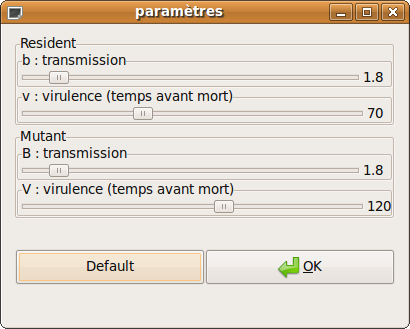
\includegraphics[width=0.4\linewidth]{graph/parametres_mutant.png}
        \caption{Séléction des paramètres pour le mutant et le résident.}
\label{fig:parametres_mutant}
\end{figure}

\textit{Evolvir} considère que les différents agents infectieux
(désigné par les noms de ``mutant'' et ``résident'') sont en
compétition directe pour les hôtes susceptibles. Si un hôte est infecté
par un des agents infectieux il n'est plus disponible pour l'autre.

Une fois les paramètres sélectionnés, le déroulement de l'épidémie
nous permet d'observer la sélection par le milieu (ici la population
humaine) des formes se reproduisant le plus (les plus adaptées)
(figure \ref{fig:mutant}). 
\begin{figure}[h!]
  \center
	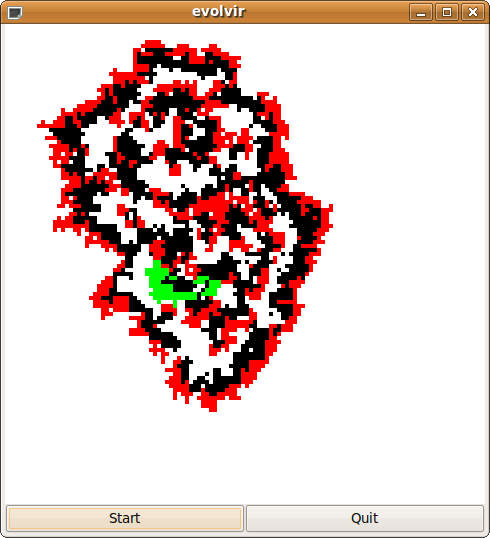
\includegraphics[width=0.4\linewidth]{graph/mutant.png}
        \caption{Apparition d'un mutant moins virulent: les individus
          infectés par le mutant sont représentés en vert.}
\label{fig:mutant}
\end{figure}

                                                                                                                
\begin{bclogo}[couleur = gray!30, logo = \bclampe , barre =                                                      
none, noborder=true ]{Simulation}                                                                                  

Choisissez différentes valeurs de paramètres pour la souche résidente
et mutante. Mémorisez bien quelle souche est la plus virulente !

Commencez ensuite la simulation en n'introduisant que la souche
résidente jusqu'à ce que la maladie soit bien établie dans la
population.

Faites alors apparaître la souches mutante et déterminez si :

\begin{itemize}
\item mutant et résident peuvent coexister ?
\item l'agent infectieux le plus virulent l'emporte ?
\item l'agent infectieux le moins virulent l'emporte ?
\end{itemize}
 
\end{bclogo}                                                                                                        

\vspace{1cm}

Cette première partie amène à la conclusion suivante : la sélection
naturelle devrait rendre tous les parasites avirulents (de virulence
nulle). En effet, lors des simulations on peut constater que, à
transmission égale, l'agent infectieux le plus virulent est toujours
remplacé par le moins virulent. Autrement dit, tout se passe comme si
la virulence était nuisible pour l'agent infectieux. On pourrait donc
conclure que tous les parasites virulents qui existent sont en fait
mal adaptés à leur hôte et, qu'avec le temps, ils devraient évoluer de
façon à perdre leur virulence. C'est ce qui a été appelé
\emph{hypothèse de la ``sagesse traditionnelle''}.

Remarquez que ce résultat est assez intuitif: un agent infectieux très
virulent tue son hôte très rapidement et donc n'a pas le temps de bien
se transmettre. Un agent infectieux tuant son hôte moins rapidement
pourra, toute chose étant égales par ailleurs, plus se transmettre et
donc exclure l'agent infectieux plus virulent en infectant tous les
hôtes potentiel.

\subsection{Confrontation à la réalité : introduction du virus de la
  myxomatose en Australie}


Le virus de la myxomatose a été introduit en Australie à partir des
années 1950 pour lutter contre la prolifération des lapins. Les lapins
avaient été introduits en Australie au milieu du XIX$^e$ siècle; ils
se répandirent rapidement dans tous le pays et furent bientôt
considérés comme des nuisibles. Différentes mesures de contrôle de la
population (incluant la chasse, l'empoisonnement, la destruction des
terriers ou l'édification de clôtures) ayant échoué, une forme très
virulente du virus de la myxomatose fut introduite au début des années
1950. Au départ, la virulence du virus a bien décliné, en accord avec
notre prédiction précédente, cependant, la suite infirma cette
hypothèse de la ``sagesse traditionnelle'' (devant rendre tous les
parasites avirulents). Au lieu de continuer leur évolution vers une
diminution de la virulence, les virus semblent s'être stabilisé à un
niveau de virulence intermédiaire. Comment expliquer le maintien de
souches virulentes dans la population de parasites ?


\subsection{Compromis évolutif entre transmission et virulence}

Jusque dans les années 80, la théorie dite de la “sagesse
traditionnelle”, était la théorie dominante en évolution de la
virulence. Roy Anderson et Robert May ont été les premiers à remettre
en cause cette théorie (en 1979) en postulant l’existence d’un
compromis évolutif entre virulence et transmission. Autrement dit:
pour pouvoir se transmettre (c’est-à-dire infecter de nouveaux hôtes)
un parasite nuit à son hôte. Exemple: pour fabriquer de nouveaux
parasites, un parasite se divise et donc utilise des ressources de son
hôte.

Transmission et virulence sont donc liés. \textit{Evolvir} permet de
s'intéresser au compromis évolutif entre virulence et transmission en
tenant compte du lien entre transmission et virulence
(figure~\ref{fig:compromis}).

\begin{figure}[h!]
  \center
	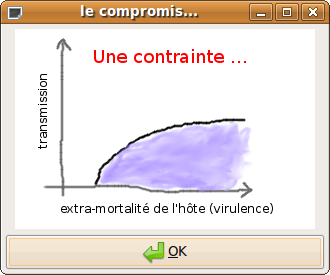
\includegraphics[width=0.4\linewidth]{graph/compromis.png}
        \caption{Compromis évolutif entre transmission et virulence.}
\label{fig:compromis}
\end{figure}

\begin{bclogo}[couleur = gray!30, logo = \bclampe , barre =                                                      
none, noborder=true ]{Simulation}                                                                                  

En sélectionant le modèle numéro 5 (compromis évolutif) lors du choix
du modèle (figure \ref{fig:selecao}), examinez les conséquences de la
prise en compte du lien entre transmission et virulence tel que décrit
par la figure~\ref{fig:compromis}.

\end{bclogo}                                                                                                        

\vspace{1cm}


La théorie du compromis introduit un dilemme pour le parasite. S’il se
transmet beaucoup, il engendre plus de nouvelles infections par unité
de temps mais tue son hôte plus vite. En revanche, s’il ménage trop
son hôte, il se transmet plus longtemps mais moins. Un peu comme
Achille, qui eut à choisir entre une vie courte mais glorieuse ou une
vie longue mais morne.

On peut ainsi montrer qu’il existe un niveau de virulence optimale
pour le parasite, qui consiste à avoir une virulence intermédiaire et
une transmission intermédiaire.

\vspace*{3cm}

\textbf{Remarque} : \textit{Evolvir} nous a permis de mieux
appréhender le déroulement d'une épidémie et certains aspects de la
théorie de l'évolution de la virulence. Il est néanmoins important de
noter que bien des hypothèses faites dans notre étude ne sont pas
toujours vérifiées dans la réalité. A titre d'exemple, un parasite est
rarement seul dans un hôte et il doit souvent le partager avec
d’autres parasites (de la même espèce ou d’une autre espèce). En
termes d’évolution de la virulence, cela est très important car la
stratégie optimale n’est plus du tout la même ! Nous n'avons pas
aborder (entre autre) les infections multiples avec \textit{Evolvir}.


\vspace*{1cm}

\begin{large}
  \textbf{Remerciements}
\end{large}

Sophie Mouge, Marion et Sissé ainsi que les classes de collèges ayant
participé aux RDV de la science 2009.


%\cite{Alizon2005}
%\cite{Ballegooijen2004}
%\cite{Frank1996}



\bibliographystyle{apalike}
\bibliography{/home/seb/Documents/biblio_bibtex/biblio_seb}

\end{document}


%%% Local Variables: 
%%% mode: latex
%%% TeX-master: t
%%% End: 
